\section{Hypothèse de robustesse}
\label{section:4.6-HYPOTHESE-ROBUSTESSE}


	%%% Introduction / Transition.
	Dans les précédentes études, nous avons presque toujours analysé le \textit{clustering} interactif en supposant que l'annotateur connaît parfaitement le domaine traité par le jeu de données et qu'il est capable de caractériser sans ambiguïté la similitude entre deux données issues de cet ensemble.
	Bien entendu, cette hypothèse forte n'est pas toujours vérifiée en situation réelle : l'interprétation du langage peut contenir certaines ambiguïtés, l'opérateur peut faire des erreurs d’inattention, et deux annotateurs peuvent avoir des avis contraire sur un même sujet.
	Dans cette section, nous nous intéresserons ainsi à la robustesse de notre méthode en présence d'erreurs d’annotation et d'incohérence dans les contraintes.
	Pour cela, nous aimerions donc vérifier l'hypothèse suivante :
	
	%%% Formulation des hypothèses:
	\begin{tcolorbox}[
		title=\faVial~\textbf{Hypothèse de robustesse}~\faVial,
		colback=colorTcolorboxHypothesis!15,
		colframe=colorTcolorboxHypothesis!75,
		width=\linewidth
	]
		% Hypothèse.
		« \textbf{
			Il est possible d'\textbf{estimer l'influence d'une différence d'annotation} lors d'une méthodologie d'annotation basée sur le \textit{clustering} interactif.
		} » \\
		
		% Figure.
		La figure~\ref{figure:4.6-HYPOTHESE-ROBUSTESSE} illustre cette hypothèse et l'espoir de estimer l'impact d'erreurs ou de différences d'annotations sur le nombre d'itérations de la méthode.
		%
		\begin{figure}[H]  % keep [H] to be in the tcolorbox.
			\centering
			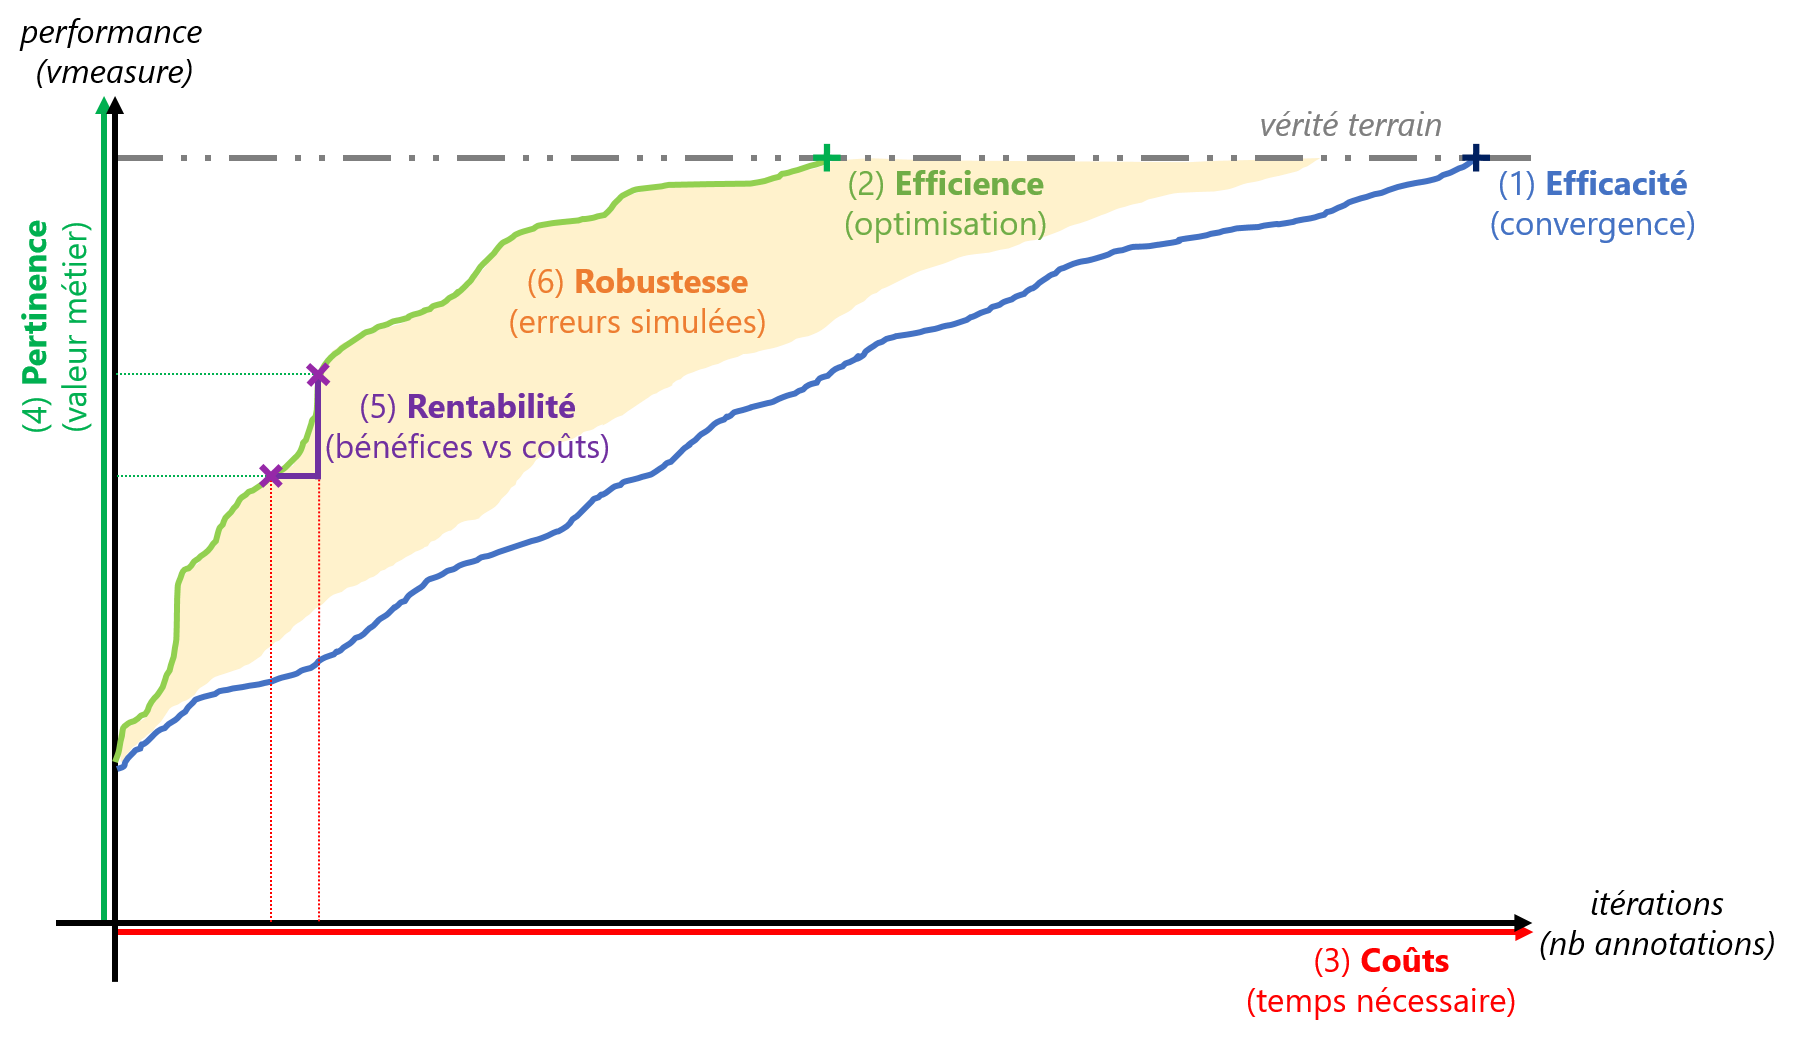
\includegraphics[width=0.95\textwidth]{figures/hypotheses-06-robustesse}
			\caption{Illustration des études réalisées sur le \textit{clustering} interactif (\textit{étape 6/6}) en schématisant l'évolution de la pertinence (\textit{valeur métier évaluée par l'expert et exprimé en nombre de clusters}) d'une base d'apprentissage en cours de construction en fonction du coût temporel de la méthode (\textit{temps nécessaire à l'expert métier et à la machine}), ainsi que les marges d'erreurs représentant l'impact de différences d'annotation sur le nombre d'itérations nécessaire à la méthode.}
			\label{figure:4.6-HYPOTHESE-ROBUSTESSE}
		\end{figure}

	\end{tcolorbox}
		
	% Résumé de l'étude.
	Afin de vérifier cette hypothèse, nous analysons l'impact d'une différence d'annotation sur les performances en simulant l'ajout de contraintes erronées, et nous discuterons de l'intérêt de prédire ou corriger les conflits d'annotation (cf. sous-section~\ref{section:4.6.1-ETUDE-ROBUSTESSE-SIMULATION-ERREURS-ANNOTATION}).
	
	
	%%%
	%%% Subsection 4.6.1: Étude de simulation d'erreurs d'annotations
	%%%
	\subsection{Étude de simulation d'erreurs d'annotations}
	\label{section:4.6.1-ETUDE-ROBUSTESSE-SIMULATION-ERREURS-ANNOTATION}
		
		% Objectif de l'expérience.
		\todo[inline]{A REDIGER: objectif de l'expérience}
	
		%%% Protocole expérimental.
		\subsubsection{Protocole expérimental}
			\todo[inline]{A REDIGER}
			% Axiome.
			% Pseudo-code.
			% Détails de l'expérience.
			
			
			% Référence scripts.
			\begin{leftBarInformation}
				Les scripts de l'expérience, réalisés avec des \textit{notebooks} Python (\cite{van-rossum-drake:2009:python-reference-manual}), sont disponibles dans un dossier dédié de~\cite{schild:2021:cognitivefactory-interactiveclusteringcomparativestudy}.
			\end{leftBarInformation}

		%%% Résultats
		\subsubsection{Résultats obtenus}
			\todo[inline]{A REDIGER}
		
			% Description statistiques.
			\todo[inline]{A REDIGER: Avec et sans corrections, avec sans sans closest.}
			
			% Figure.
			%
			\begin{figure}[!htb]
				\centering
				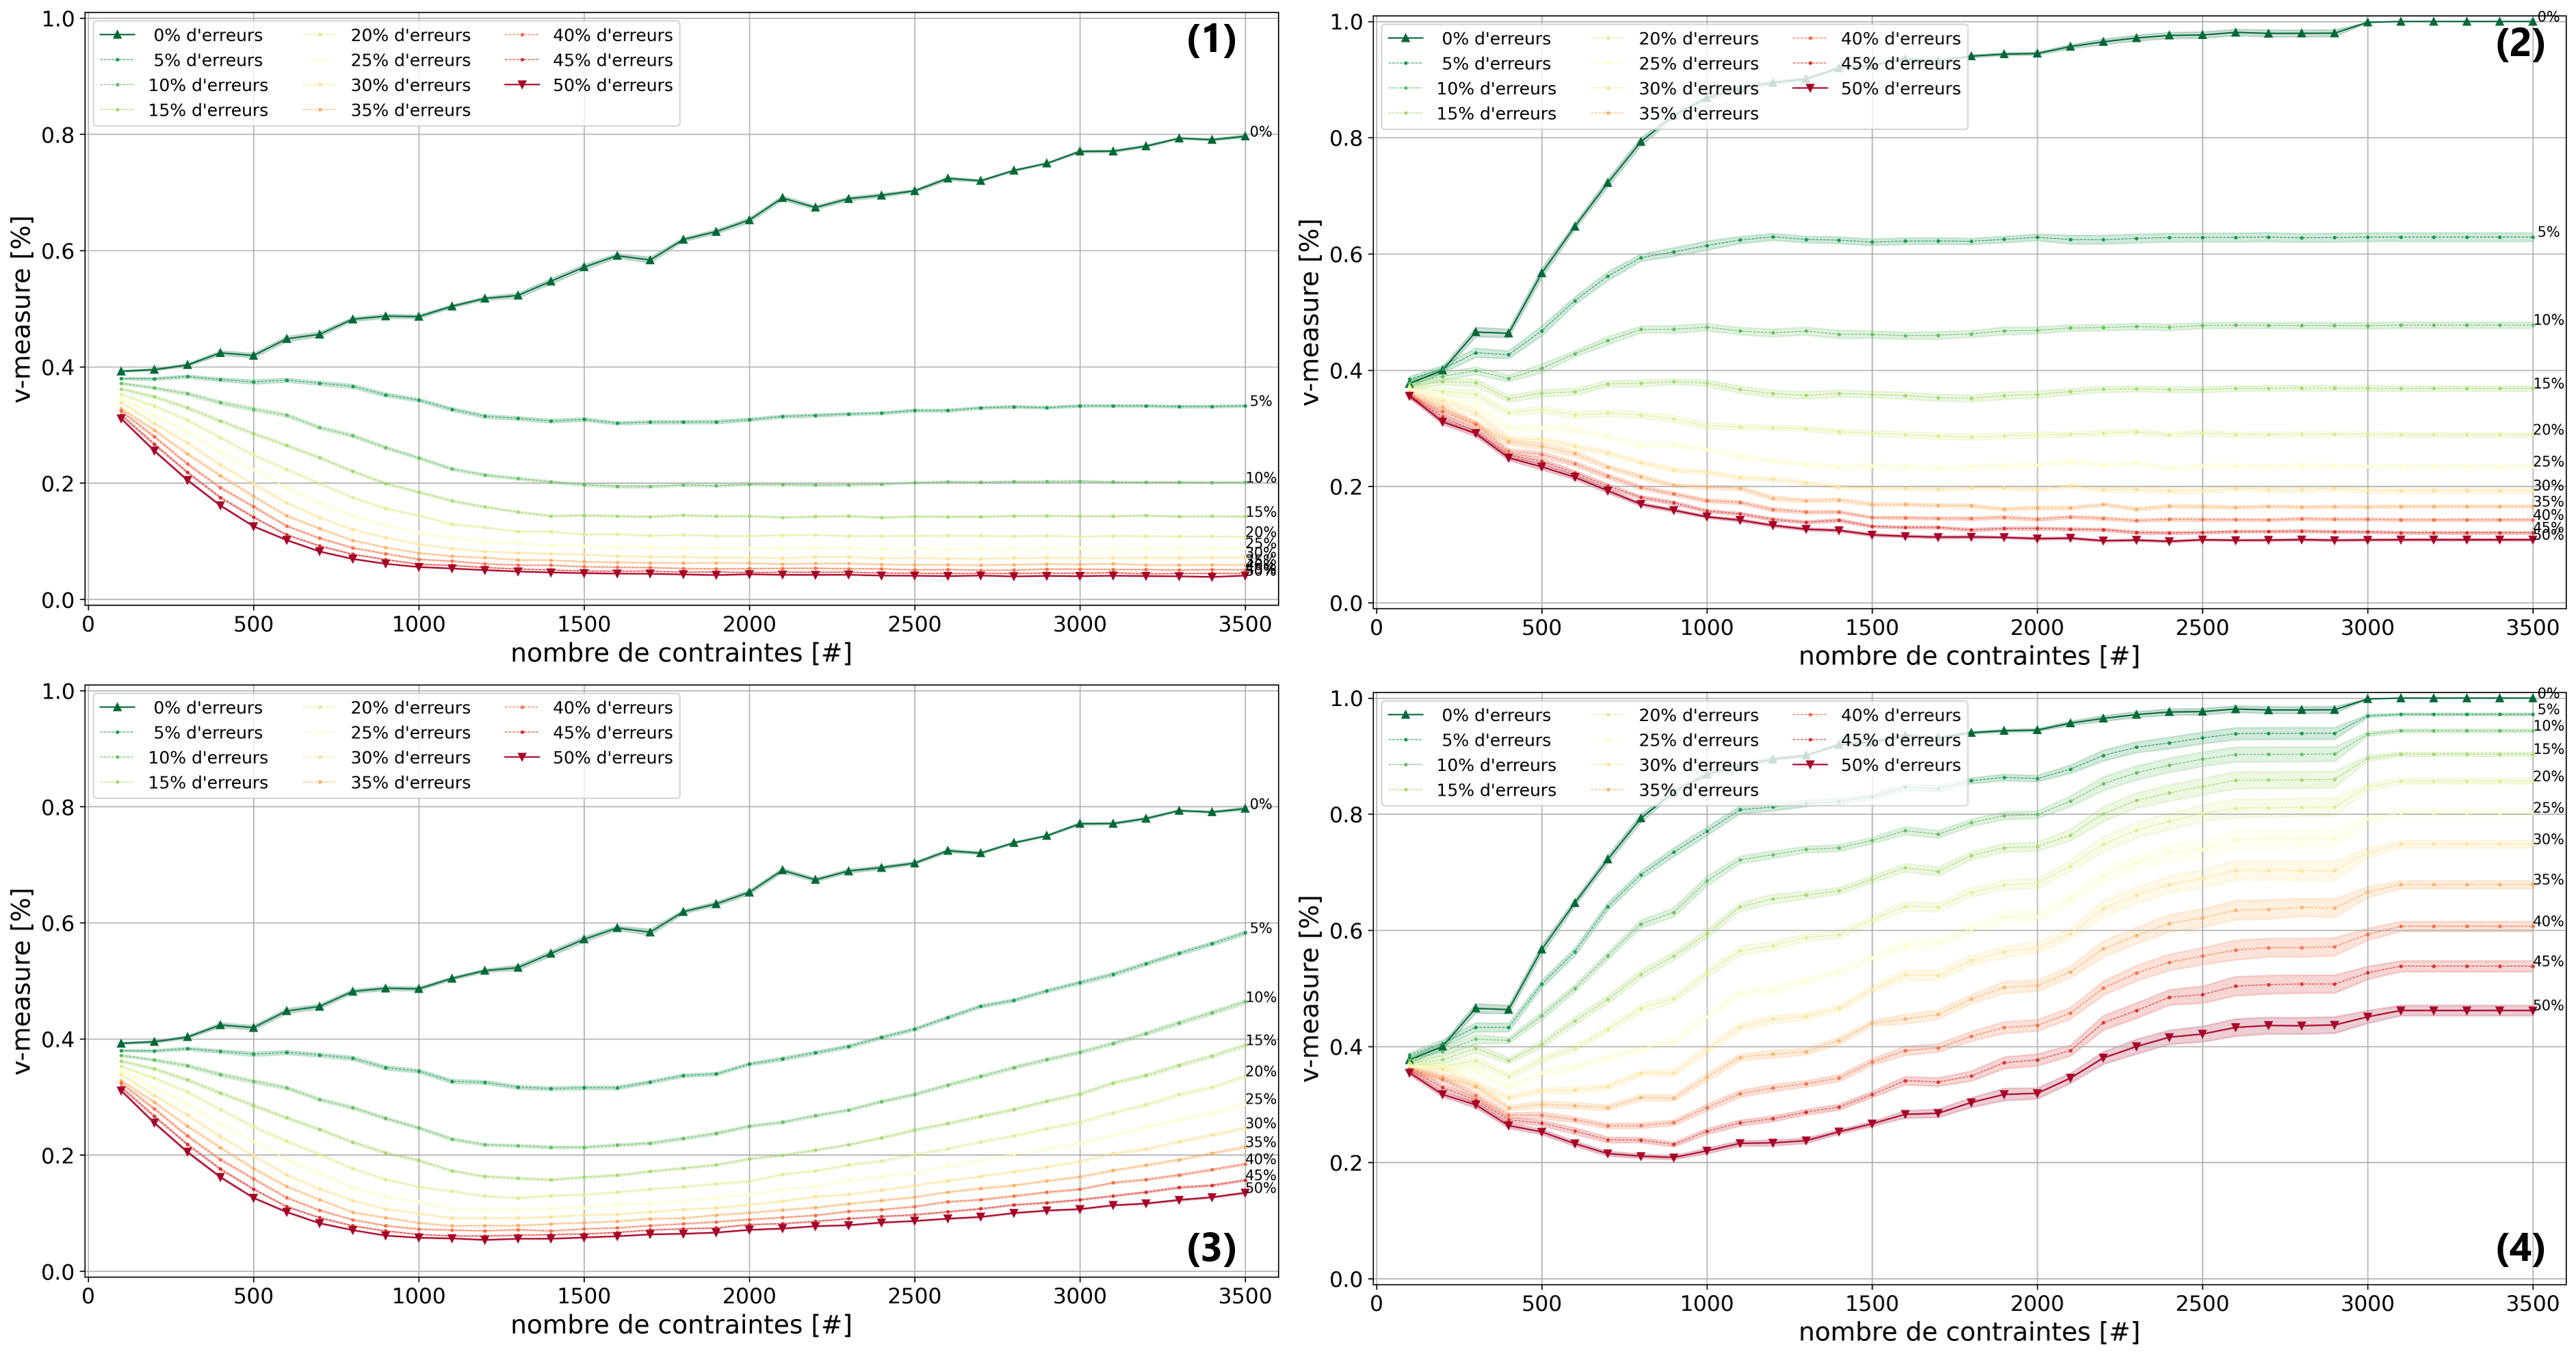
\includegraphics[width=0.95\textwidth]{figures/etude-erreur-simulation-impact}
				\caption{Évolutions de la moyenne de la \texttt{v-measure} entre un résultat obtenu et la vérité terrain en fonction du nombre d'itération de la méthode de \textit{clustering} interactif, moyenne prenant en compte différents taux d'erreurs d'annotations entre $0$ et $50$\%.}
				\label{figure:4.6.1-ETUDE-ROBUSTESSE-SIMULATION-ERREURS-ANNOTATION}
			\end{figure}

		%%% Discussion
		\subsubsection{Discussion}
			\todo[inline]{A REDIGER}
		
			% Remaques expérience utilisateur.
			\todo[inline]{A REDIGER: Super important de corriger}
			
			% Conclusions et suggestion.
	
	
	%%%
	%%% Subsection 4.6.2: Étude d'annotation avec des paradigmes différents
	%%%
	%\subsection{Étude d'annotation avec des paradigmes différents}
	%\label{section:4.6.2-ETUDE-ROBUSTESSE-ANNOTATIONS-DIFFERENTES}
	%	
	%	% Objectif de l'expérience.
	%	\todo[inline]{A REDIGER: objectif de l'expérience}
	%
	%	%%% Protocole expérimental.
	%	\subsubsection{Protocole expérimental}
	%		\todo[inline]{A REDIGER}
	%		% Axiome.
	%		% Pseudo-code.
	%		% Détails de l'expérience.
	%		% Référence scripts.
	%
	%	%%% Résultats
	%	\subsubsection{Résultats obtenus}
	%		\todo[inline]{A REDIGER}
	%	
	%		% Description statistiques.
	%		
	%		% Exemple.
	%
	%	%%% Discussion
	%	\subsubsection{Discussion}
	%		\todo[inline]{A REDIGER}
	%	
	%		% Remaques expérience utilisateur.
	%		
	%		% Conclusions et suggestion.